\section{Results}\label{sec:results}

Every closed-form expression derived above is first validated against an exact
continuous-time Markov chain (CTMC), then used to compare the solved models and quantify
the two mechanisms.

\subsection{Validation against the CTMC}\label{subsec:validation}

The ground truth is a truncated CTMC solver: it solves the linear system $\pi Q=0$ directly,
with no approximation beyond the finite truncation at $N_{\max}=40$. Each theoretical result
--- two lemmas, three theorems, two corollaries, one approximation theorem, and two
experiment-model theorems --- is verified against the exact stationary distribution at base
parameters $\lambda_1=0.3$, $\lambda_2=0.4$, $\mu=1.0$, with the mechanism parameter
($\gamma_1$ or $\theta_1$) set to $0.5$ where applicable.

Table~\ref{tab:validation_summary} collects the verdict for every result. All mathematical
results are accepted to within CTMC truncation noise: the lemma residuals and closed-form
PGF errors fall between $10^{-7}$ and $10^{-15}$, and the corollary scatter lies on the
diagonal to $10^{-4}$ across $60$ random configurations each. A discrete-event simulation of
the master chain cross-validates the CTMC itself to the $O(1/\sqrt{n})$ sampling floor.

% ─────────────────────────────────────────────────────────────────────────────
\begin{table}[H]
\centering
\caption{Validation summary.  All mathematical results are accepted; the PPGF
approximation is conditionally accepted (accurate only for $\rho_1/\rho\ge0.6$
and $\rho\le0.6$).  Max errors reflect CTMC truncation, not formula error.}
\label{tab:validation_summary}
\renewcommand{\arraystretch}{1.35}
\footnotesize
\begin{tabular}{llllcl}
\hline
\textbf{ID} & \textbf{Result} & \textbf{Model(s)} & \textbf{Check} & \textbf{Max error} & \textbf{Verdict} \\
\hline
L1   & Lemma~\ref{lem:gen:fundamental_equation}  & A, B, B$_2$, C$_2$ & PGF eq.\ residual             & $<5\times10^{-9}$  & Accept \\
L2   & Lemma~\ref{lem:gen:PPGF_dynamics}         & A, B$_2$, C$_2$    & PPGF dynamics residual        & $<2\times10^{-15}$ & Accept \\
T-A  & Theorem~\ref{thm:A:PGF}                     & A                  & $P(x,y)$ on $5\times5$ grid   & $<4\times10^{-8}$  & Accept \\
C-A  & Corollary~\ref{cor:A:pi0}                 & A, B, B$_2$        & $\pi_0$, $\pi(0,0)$, 60 configurations  & $<10^{-4}$         & Accept \\
T-B2 & Theorem~\ref{thm:B2:PGF}                  & B$_2$              & $P(x,y)$ on $5\times5$ grid, $x<y$   & $<3\times10^{-7}$  & Accept \\
T-C2 & Theorem~\ref{thm:C2:PGF}                  & C$_2$              & $P(x,y)$ on $5\times5$ grid   & $<5\times10^{-12}$ & Accept \\
C-C2 & Corollary~\ref{cor:C2:pi00}               & C$_2$              & $\pi_0$, $\pi(0,0)$, 60 configurations  & $<10^{-4}$         & Accept \\
T-S  & Approximation~\ref{apx:A:PPGF_Stilde}     & A                  & $\varepsilon_\infty$ over $(\rho_1,\rho_2)$ & $0$--$100\%$ & Conditional \\
\hline
E-B  & Theorem~\ref{thm:B21:PGF} — Model-$\BH$  & $\BH$            & $P(x,y)$ on $5\times5$ grid                 & $<3\times10^{-7}$  & Accept \\
E-C  & Theorem~\ref{thm:C21:PGF} — Model-$\CH$ & $\CH$            & $P(x,y)$ on $5\times5$ grid                 & $<3\times10^{-11}$ & Accept \\
\hline
\end{tabular}
\end{table}

A single entry is only conditionally accepted. The partial-PGF recursion on the alternative
state space $\widetilde{S}$ (Approximation~\ref{apx:A:PPGF_Stilde}) is approximate by design:
it drops the boundary-diagonal forcing term, so it is exact at $y=1$ but degrades elsewhere.
It is reliable only in the priority-dominated, moderately loaded regime
($\rho_1/\rho\gtrsim0.6$, $\rho\lesssim0.6$).

\subsection{Comparison of the solved models}
\label{sec:comparison}

With every closed form validated, we compare the five solved models: the baseline ($A$), the
jockeying extension ($B_2$), the abandonment extension ($C_2$), and their head-of-line
variants ($\BH$, $\CH$). The first three are the tractable specialisations of Model-$X$;
the head-of-line variants are the standalone simplifications of
\S\S\ref{sec:model_b21}--\ref{sec:model_c21}. Each produces a closed-form or integral-form
expression for $P(x,y)$. Table~\ref{tab:comparison} collects the key structural facts for the
three full-rate models.

\begin{table}[H]
\centering
\caption{Structural comparison of Models $A$, B$_2$, and C$_2$.}
\label{tab:comparison}
\renewcommand{\arraystretch}{1.4}
\begin{tabular}{p{0.26\textwidth} p{0.21\textwidth} p{0.21\textwidth} p{0.21\textwidth}}
\hline
 & \textbf{Model-$A$} & \textbf{Model-$B_2$} & \textbf{Model-$C_2$} \\
\hline
Extra mechanism
 & none
 & jockeying $1\!\to\!2$ ($\gamma_1>0$)
 & class-1 abandonment ($\theta_1>0$) \\
Stability condition
 & $\rho<1$
 & $\rho<1$
 & $\rho_2\cdot{}_1F_1<1$ \\
Fundamental equation
 & algebraic PGF equation
 & 1st-order PDE in $x,y$
 & 1st-order ODE in $x$ \\
Pinning of $P_y(y)$
 & zero of kernel: $x=x^*(y)$
 & analyticity at $x=y$
 & boundedness at $x=1$ \\
Probabilistic route
 & yes (P-K with $B$)
 & no (jockeying breaks Poisson)
 & yes (P-K with $B_C$) \\
$P_y(y)$
 & rational in $x^*(y)$
 & Kummer ratio \eqref{eq:B2:Py}
 & P-K / Kummer \eqref{eq:C2:Py} \\
$P(x,y)$
 & closed form \eqref{eq:A:fundamental}
 & integral form \eqref{eq:B2:Pxy}
 & integral form \eqref{eq:C2:Pxy} \\
$\pi(0,0)$
 & $\rho(1-\rho)$
 & $\rho(1-\rho)$
 & $(\rho_1{+}\rho_2)\pi_0$ via $\mathbb{E}[B_C]$ \\
$\pi_0$
 & $1-\rho$
 & $1-\rho$
 & $>1-\rho$ (abandonment increases idle time) \\
$P(z,z)$
 & $\rho(1-\rho)/(1-\rho z)$
 & $\rho(1-\rho)/(1-\rho z)$
 & no closed form \\
\hline
\end{tabular}
\end{table}

\subsubsection*{Model-\texorpdfstring{$A$}{A}: the rational baseline}

Model-$A$ imposes no extra departure mechanism.
Class-1 operates as an independent $M/M/1(\lambda_1,\mu)$ queue;
class-2 sees an $M/G/1$ with service time equal to a class-1 busy period
(by PASTA and the priority decomposition of \S\ref{ssec:priority}).
The Pollaczek--Khinchine formula~\eqref{eq:pk:pgf} delivers $P_y(y)$
as a rational function of $x^*(y)$, and $P(x,y)$ is a ratio of polynomials
in $x$, $y$, and $x^*(y)$.  All performance measures --- $\pi_0$, $\pi(0,0)$,
$\mathbb{E}[N_i]$, $\mathbb{E}[W_i]$ --- are in closed form.  Model-$A$ also
furnishes the structural identities that persist across the hierarchy:
$P(z,z)=\rho(1-\rho)/(1-\rho z)$ (total queue is $M/M/1$),
$\pi_0=1-\rho$, and $\pi(0,0)=\rho(1-\rho)$.

\subsubsection*{Effect of jockeying: Model-\texorpdfstring{$A$}{A} \texorpdfstring{$\to$}{->} Model-\texorpdfstring{$B_2$}{B2}}

Adding one-way jockeying ($\gamma_1>0$, $\gamma_2=0$) couples the two queues:
a class-1 customer waiting in Queue~1 may defect to Queue~2 at rate $\gamma_1$.
The consequences are asymmetric.

\emph{What is preserved.}
Jockeying transfers customers but does not remove them, so the total-customer
process remains a standard $M/M/1(\lambda,\mu)$ birth--death chain.
Consequently $P(z,z)$, $\pi_0$, $\pi(0,0)$, and $\mathbb{E}[N]$ are identical
to Model-$A$ for all $\gamma_1>0$.

\emph{What is destroyed.}
Jockeying breaks the per-class Poisson/renewal structure: a class-2 customer
can no longer identify its effective service time with a class-1 busy period.
The P-K route is therefore unavailable.

\emph{What is new.}
The fundamental PGF equation gains the convection term
$\gamma_1 xy(x-y)\partial_x P$, which reduces it to a first-order ODE in $x$
for each fixed $y$ (since $\gamma_2=0$ kills the $\partial_y$ term).
The solution closes via an integrating factor with a branch singularity at the
\emph{interior} point $x=y$; the branch coefficient must vanish for $P$ to be
holomorphic, and this analyticity condition pins $P_y(y)$ as a Kummer ratio.
The individual means $\mathbb{E}[N_1]$ and $\mathbb{E}[N_2]$ change with
$\gamma_1$ (class-1 becomes shorter, class-2 longer), with no closed form for
the split.

\subsubsection*{Effect of abandonment: Model-\texorpdfstring{$A$}{A} \texorpdfstring{$\to$}{->} Model-\texorpdfstring{$C_2$}{C2}}

Adding class-1 abandonment ($\theta_1>0$, $\theta_2=0$, $\gamma_i=0$)
allows each waiting class-1 customer to leave the system at rate $\theta_1$.

\emph{What is preserved.}
Class-2 customers still see Poisson arrivals (abandonment only affects
class-1; the class-2 arrival process is undisturbed).
PASTA therefore still applies, and the $M/G/1$ subsystem for class-2 is
intact --- now with effective service time $B_C$ (the busy period of the
$M/M/1+M$ queue of \S\ref{ssec:erlangA}) replacing $B$.
The P-K formula~\eqref{eq:pk:pgf} applies with $B_C$ and delivers $P_y(y)$.

\emph{What is destroyed.}
Abandonment is a true departure: it reduces the total number of customers and
breaks the conservation property.  Consequently $P(z,z)$ no longer has the
simple $M/M/1$ form of Corollary~\ref{cor:A:pi0}, $\pi_0>1-\rho$, $\pi(0,0)$ requires
$\mathbb{E}[B_C]$, and $\mathbb{E}[N]<\rho^2/(1-\rho)$.  The stability
condition is also generalised: $\rho<1$ is no longer necessary; the relevant
condition is $\lambda_2\,\mathbb{E}[B_C]<1$, which is strictly weaker for all
$\theta_1>0$.

\emph{What is new.}
The fundamental equation gains the convection term
$\theta_1 xy(x-1)\partial_x P$, which already reduces it to a first-order ODE
in $x$ for each fixed $y$ (with $\theta_2=0$ killing the $\partial_y$ term).
The integrating factor now has its singularity at the \emph{boundary} $x=1$
with a positive exponent, so $\mu_I$ vanishes there and mere boundedness of
$P$ forces $\int_0^1 q\,\mu_I\,dt=0$.  This determines $P_y(y)$ without any
reference to holomorphy.  Both $\mathbb{E}[N_1]$ and $\mathbb{E}[N_2]$ decrease
relative to Model-$A$ as $\theta_1$ increases: class-2 benefits indirectly
because class-1 abandonments free the server sooner.

\subsubsection*{Structural comparison of Models \texorpdfstring{$B_2$}{B2} and C\texorpdfstring{$_2$}{2}}

Both models reduce the fundamental equation to a first-order linear ODE in $x$
and both close in confluent hypergeometric functions; yet the mechanism that
pins $P_y(y)$ is structurally different.

\begin{center}
\renewcommand{\arraystretch}{1.45}
\begin{tabular}{p{0.28\textwidth} p{0.31\textwidth} p{0.31\textwidth}}
\hline
 & \textbf{Model-$C_2$ ($\theta_1>0$)} & \textbf{Model-$B_2$ ($\gamma_1>0$)} \\
\hline
Convection coefficient
 & $\theta_1\,x(x-1)$
 & $\gamma_1\,x(x-y)$ \\
Operative singular point
 & boundary $x=1$
 & interior $x=y$ \\
Exponent at singularity
 & $\beta(y)=\lambda_2(1-y)/\theta_1>0$ \;($\mu_I\to0$)
 & $\beta(y)=(1-y)(\lambda y-\mu)/(\gamma_1 y)<0$ \;($\mu_I\to\infty$) \\
Pinning principle
 & \emph{boundedness}: $\int_0^1 q\,\mu_I\,dt=0$
 & \emph{analyticity}: branch coefficient $=0$ \\
$\pi(0,0)$
 & $M/G/1{+}$renewal (conservation broken)
 & $\rho(1-\rho)$ exactly (conservation holds) \\
Probabilistic backbone
 & class-$2$ is $M/G/1$; P-K with $B_C$
 & class-$1$ is $M/M/1{+}M$ (reneging $=\gamma_1$); no P-K \\
\hline
\end{tabular}
\end{center}

In words: in Model-$C_2$ the singularity sits on the boundary $x=1$ with a positive
exponent, so $\mu_I$ vanishes and mere boundedness pins $P_y(y)$; the class-2 stream stays
Poisson, so P-K and an $M/G/1$ renewal argument deliver $P_y(y)$ and $\pi(0,0)$. In
Model-$B_2$ the singularity sits at the interior point $x=y$ with a negative exponent, so
$\mu_I$ blows up and only holomorphy --- the absence of the branch $(x-y)^{|\beta|}$ --- pins
$P_y(y)$. Jockeying leaves no P-K identity; the $M/M/1{+}M$ reading of the class-1 marginal is
the origin of the ${}_1F_1$ factors.

\subsubsection*{Common Erlang-A structure}

A common object appears in both B$_2$ and C$_2$:
\begin{equation}
    {}_1F_1\!\left(1;\,\frac{\mu}{r}+1;\,\frac{\lambda_1}{r}\right),
    \label{eq:comp:1F1}
\end{equation}
with $r=\gamma_1$ (Model-$B_2$) or $r=\theta_1$ (Model-$C_2$).
This is the Erlang-A utilisation factor: in C$_2$ it equals $\mu\,\mathbb{E}[B_C]$, while in
B$_2$ it controls the Kummer ratio in $P_y(y)$ through the exponent $\alpha(y)=\mu/(\gamma_1 y)$.
In both cases the function evaluates at a negative argument
$(-\lambda_1/r)$ in C$_2$ and $(-\lambda_1 y/\gamma_1)$ in B$_2$, and the
ratio ${}_1F_1(\alpha+1;\cdot;\cdot)/{}_1F_1(\alpha;\cdot;\cdot)$ acts as a
boundary correction to the Model-$A$ rational formula.

Model-$B_2$ degenerates to Model-$A$ only in the singular limit
$\gamma_1\to0^+$, in which $\alpha,\beta\to\infty$ and the Kummer ratio
collapses to the rational expression $x^*(y)(1-y)/(x^*(y)-y)$ of Model-$A$.
This limit is not uniform, consistent with $\gamma_1$ multiplying the
highest-order term of the ODE.  Model-$C_2$ degenerates to Model-$A$ uniformly
as $\theta_1\to0^+$: $\mathbb{E}[B_C]\to(\mu-\lambda_1)^{-1}$, and all
C$_2$ formulas recover their Model-$A$ counterparts.

% ─────────────────────────────────────────────────────────────────────────────
\subsubsection{Quantitative comparison across load}
\label{subsec:comp:sweep}

Holding $\mu=1$ and the arrival split fixed at $\lambda_1{:}\lambda_2=3{:}4$, we sweep the offered
load $\rho$ across $[0.10,0.95]$ and compute the exact stationary performance of the five solved
models on the truncated CTMC. Figure~\ref{fig:comp:sweep_en} plots $\mathbb{E}[N]$,
$\mathbb{E}[N_1]$, $\mathbb{E}[W_1]=\mathbb{E}[N_1]/\lambda_1$ (Little's Law), and $\pi_0$;
Table~\ref{tab:comp:main} reads off the full descriptor set at three reference loads.

%% BEGIN SIMULATION RESULTS — fig_sweep_EN_vs_rho %%
\begin{figure}[H]
  \centering
  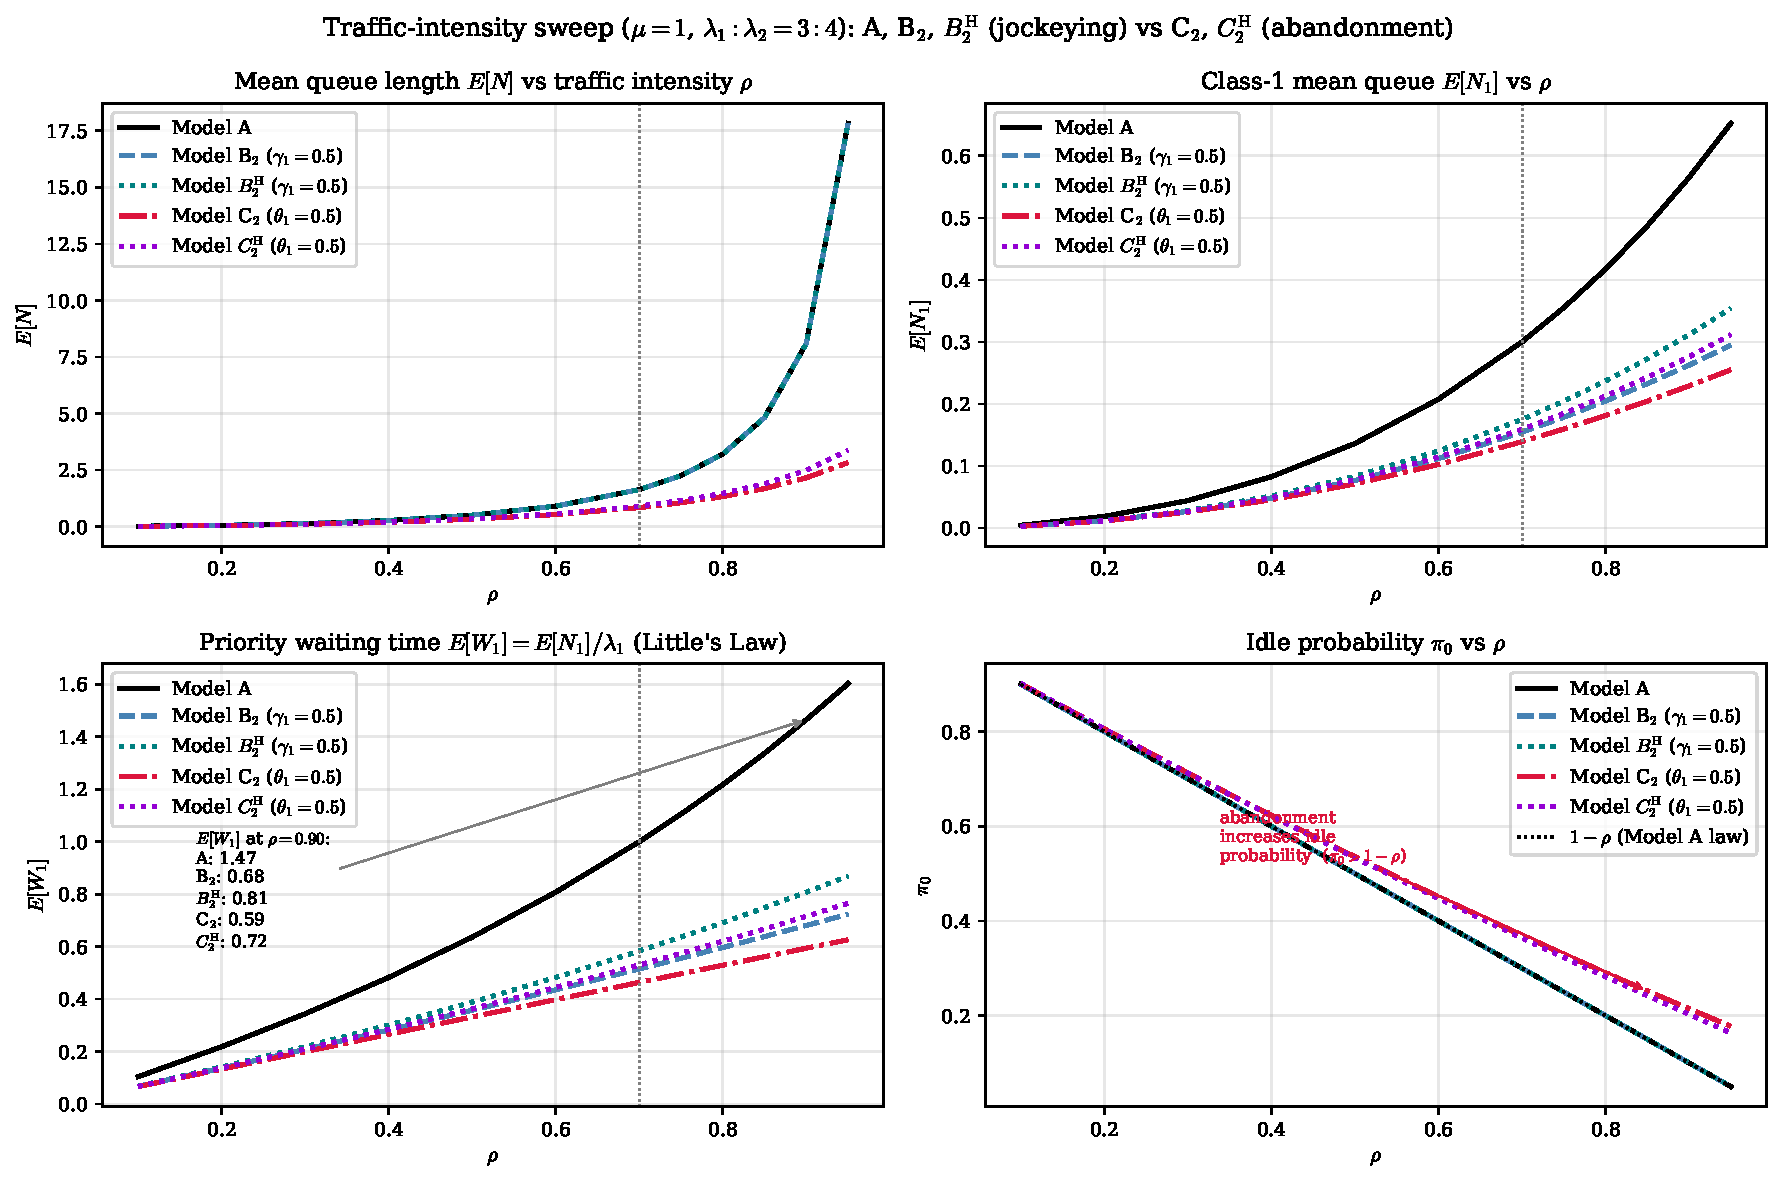
\includegraphics[width=0.98\textwidth]{figures/results/fig_sweep_EN_vs_rho.pdf}
  \caption{Performance versus traffic intensity $\rho$ for the five solved models ---
  the baseline $A$, the jockeying pair $B_2$, $\BH$ ($\gamma_1=0.5$), and the
  abandonment pair $C_2$, $\CH$ ($\theta_1=0.5$) --- at $\mu=1$ and
  $\lambda_1{:}\lambda_2=3{:}4$; the vertical line marks the canonical $\rho=0.70$.
  \emph{Top-left:} total queue $\mathbb{E}[N]$ --- $A$, $B_2$ and $\BH$ coincide because
  jockeying conserves $N$ (Corollaries~\ref{cor:A:pi0}, \ref{cor:B21:pi0}), while $C_2$ and
  $\CH$ lie strictly below because abandonment removes customers ($\CH$ by less).
  \emph{Top-right:} priority queue $\mathbb{E}[N_1]$ --- the head-of-line variants drain it
  less than their full-rate cousins. \emph{Bottom-left:} priority waiting time
  $\mathbb{E}[W_1]$. \emph{Bottom-right:} idle probability $\pi_0$, with the $1-\rho$ law
  (Models~$A$, $B_2$, $\BH$) shown dotted; $C_2$ and $\CH$ sit above it for every $\rho$,
  as predicted by Corollaries~\ref{cor:C2:pi00}, \ref{cor:C21:pi0}.}
  \label{fig:comp:sweep_en}
\end{figure}
%% END SIMULATION RESULTS — fig_sweep_EN_vs_rho %%

%% BEGIN SIMULATION RESULTS — tab_comparison_main %%
\begin{table}[t]\centering
\caption{Comparison of Models $A$, $B$ ($\gamma_1=0.5$, $\gamma_2=0.3$), $B_2$ and $\BH$ ($\gamma_1=0.5$), and $C_2$ and $\CH$ ($\theta_1=0.5$) at three traffic intensities with $\lambda_1{:}\lambda_2=3{:}4$, $\mu=1$. The head-of-line models $\BH$ and $\CH$ use the rate $\gamma_1\mathbf{1}_{\{n_1\geq1\}}$, respectively $\theta_1\mathbf{1}_{\{n_1\geq1\}}$; Model-$B_2$ and Model-$C_2$ use the full rates $\gamma_1 n_1$ and $\theta_1 n_1$. Model-$B$, whose PGF remains open, joins through its truncated-CTMC solution ---like every entry of this table--- since no closed form is required for the comparison.}
\label{tab:comp:main}
\begin{tabular}{llrrrrrrr}
\toprule
$\rho$ & Model & $E[N_1]$ & $E[N_2]$ & $E[N]$ & $E[W_1]$ & $E[W_2]$ & $\pi_0$ & $\pi(0,0)$ \\
\midrule
\multirow{6}{*}{0.50} & $A$ & 0.1364 & 0.3636 & 0.5000 & 0.6364 & 1.2727 & 0.5000 & 0.2500 \\
 & $B$ & 0.1665 & 0.3335 & 0.5000 & 0.7772 & 1.1671 & 0.5000 & 0.2500 \\
 & $B_2$ & 0.0767 & 0.4233 & 0.5000 & 0.3578 & 1.4817 & 0.5000 & 0.2500 \\
 & $\BH$ & 0.0833 & 0.4167 & 0.5000 & 0.3889 & 1.4583 & 0.5000 & 0.2500 \\
 & $C_2$ & 0.0712 & 0.2521 & 0.3233 & 0.3323 & 0.8823 & 0.5356 & 0.2678 \\
 & $\CH$ & 0.0778 & 0.2593 & 0.3370 & 0.3630 & 0.9074 & 0.5333 & 0.2667 \\
\midrule
\multirow{6}{*}{0.70} & $A$ & 0.3000 & 1.3333 & 1.6333 & 1.0000 & 3.3333 & 0.3000 & 0.2100 \\
 & $B$ & 0.5149 & 1.1184 & 1.6333 & 1.7164 & 2.7961 & 0.3000 & 0.2100 \\
 & $B_2$ & 0.1545 & 1.4788 & 1.6333 & 0.5151 & 3.6970 & 0.3000 & 0.2100 \\
 & $\BH$ & 0.1750 & 1.4583 & 1.6333 & 0.5833 & 3.6458 & 0.3000 & 0.2100 \\
 & $C_2$ & 0.1392 & 0.6967 & 0.8358 & 0.4639 & 1.7417 & 0.3696 & 0.2587 \\
 & $\CH$ & 0.1591 & 0.7424 & 0.9015 & 0.5303 & 1.8561 & 0.3636 & 0.2545 \\
\midrule
\multirow{6}{*}{0.90} & $A$ & 0.5651 & 7.5346 & 8.0997 & 1.4651 & 14.6506 & 0.1000 & 0.0900 \\
 & $B$ & 2.6711 & 5.4289 & 8.1000 & 6.9250 & 10.5563 & 0.1000 & 0.0900 \\
 & $B_2$ & 0.2626 & 7.8371 & 8.0997 & 0.6808 & 15.2388 & 0.1000 & 0.0900 \\
 & $\BH$ & 0.3115 & 7.7882 & 8.0997 & 0.8077 & 15.1437 & 0.1000 & 0.0900 \\
 & $C_2$ & 0.2292 & 1.9245 & 2.1537 & 0.5941 & 3.7421 & 0.2146 & 0.1931 \\
 & $\CH$ & 0.2760 & 2.2084 & 2.4844 & 0.7157 & 4.2941 & 0.2025 & 0.1823 \\
\bottomrule
\end{tabular}
\end{table}

%% END SIMULATION RESULTS — tab_comparison_main %%

The two mechanisms produce two qualitatively different responses. Jockeying is internal: the
$1\!\to\!2$ transition relabels a waiting customer without changing the total count. The
$B_2$ and $A$ curves for $\mathbb{E}[N]$ and $\pi_0$ are therefore indistinguishable across the entire
sweep --- the server sees the same workload, and the busy-but-empty probability stays on the
$\rho(1-\rho)$ parabola of Corollary~\ref{cor:B2:pi00}. Abandonment is a true departure at
rate $\theta_1 n_1$, so $C_2$ carries a strictly lighter queue and a strictly larger idle
fraction: the priority backlog is bled off before it can be served. At $\rho=0.70$
(Table~\ref{tab:comp:main}) this gives $\pi_0=\piZeroCtwoSeventy$ for $C_2$ against $\piZeroASeventy$ for $A$ and
$B_2$, and $\mathbb{E}[N]=\ENCtwoSeventy$ against $\ENASeventy$. The divergence widens with load: at
$\rho=0.90$ the baseline class-2 queue reaches $\mathbb{E}[N_2]=\ENtwoANinety$, whereas $C_2$ holds
it to $\ENtwoCtwoNinety$ --- a factor of nearly four. The self-regulating valve $\theta_1 n_1$
acts most strongly precisely when the queue is long. The two head-of-line variants interpolate
monotonically between Model-$A$ and their full-rate parents in every descriptor: $\BH$ conserves
$N$ exactly like $B_2$ and departs only in the $\mathbb{E}[N_1]$ split, while $\CH$ sheds less
load than $C_2$ ($\pi_0=\piZeroCHSeventy$, $\mathbb{E}[N]=\ENCHSeventy$ at $\rho=0.70$).

Two columns warrant a reviewer's caution. First, $\mathbb{E}[W_1]$ is smallest for $C_2$ at
every load, but $\mathbb{E}[W_i]=\mathbb{E}[N_i]/\lambda_i$ counts residence in queue~$i$, which
every departure mode shortens --- service \emph{and} attrition. A smaller $\mathbb{E}[W_1]$ thus
does not certify faster service. Second, jockeying actively \emph{harms} class~2: at $\rho=0.70$,
$B_2$ raises $\mathbb{E}[W_2]$ to $\EWtwoBtwoSeventy$ from the baseline $\EWtwoASeventy$
($+\EWtwoBtwoInflationSeventy\%$). Finally, near criticality the dense CTMC truncation leaves a
boundary tail mass of order $6\times10^{-4}$ for $A$ and $B_2$ at $\rho=0.95$ (against
$1.5\times10^{-7}$ for $C_2$), so the $\rho\ge0.92$ points for the non-abandoning models are
lower bounds.


% ─────────────────────────────────────────────────────────────────────────────
\subsection{Convergence to the baseline}\label{subsec:results:convergence}

Each specialised model must recover Model-$A$ as its distinguishing parameter vanishes; the
comparison above establishes this algebraically, and the CTMC pipeline confirms it numerically.
Measured in the $L_1$ distance $\lVert\pi-\pi_A\rVert_1$, all four specialised models ---
$B_2$, $C_2$, $\BH$, $\CH$ --- approach the baseline at first order in their distinguishing
parameter, with fitted log--log slopes of $0.85$--$0.93$. For the conserving models $B_2$ and
$\BH$ the empty-state descriptors $\pi_0$ and $\pi(0,0)$ equal their Model-$A$ values
\emph{identically} for every $\gamma_1>0$ (Corollaries~\ref{cor:B2:pi00}, \ref{cor:B21:pi0}),
so the approach is carried entirely by interior redistribution of mass.
